\subsection{Auswertung Modellwahl}
Tats\"achlich schneidet im Vergleich zu den anderen drei Herangehensweisen die explorative am besten ab, wie anhand von Tabelle \ref{tab:wic} und Abbildung \ref{fig:wic} nachvollzogen werden kann.
Dies liegt aber auch vor allem daran, dass \textsc{mExplorativ} die geringste Anzahl an Eingabevariablen besitzt.

\begin{table}[ht]
\centering
\begin{tabular}{rrrrrr}
  \hline
  & name & df & AIC & $\hat{SPSE}$ & Devienz  \\ 
  \hline
	1 & mExplorativ & 16.00 & 1405.77 & 0.9999914 & 92.27836 \\ 
	2 & mEinzeln & 8.00 & 1468.70 &  0.999921 & 94.33151\\   
  	3 & mStep & 9.00 & 1457.60 &  1 & 94.97083\\ 
    4 & mCor & 7.00 & 1472.06 &  0.9999654 & 95.23178\\ 
   \hline
\end{tabular}
\caption{Kriterien der vier Gewinnermodelle}
\label{tab:wic}
\end{table}

\begin{figure}
\centering
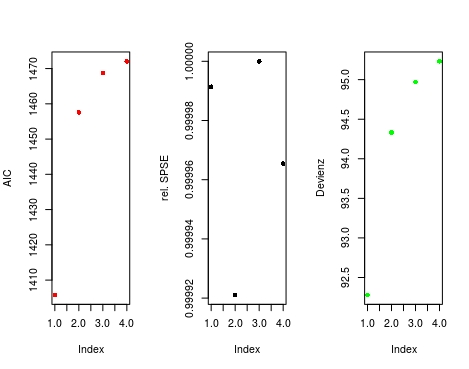
\includegraphics[scale=1]{./jpgs/wic.jpeg}
\caption{Graphische Veranschaulichung der verschiedenen Korrelationswerte.}
\label{fig:wic}
\end{figure} 
Zur Modellwahl muss gesagt werden, dass ein recht gutes Ergebnis mit \textdc{mExplorativ} gefunden wurde.
Auch die anderen gefundenen 'Siegermodelle' sind entsprechend gut.
Anhand der vorgestellten Herangehensweisen k\"onnen also Modelle gefunden werden, welche gute Sch\"atzungen liefern. \\
Zu Beginn der Untersuchung wurde auch die Zielvariable ver\"andert: \\
Statt \textit{crimes} wurden die Werte \text{crimes-per-area} ($cpa$) benutzt.
\begin{equation}
cpa = \frac{crimes}{area}
\end{equation}
Dadurch wurden sehr geringe Werte f\"ur die Kriterien ermittelt.
Dies liegt wohl aber auch an den wesentlich kleineren Bereich, in dem sich dann die Zielgr\"s\ss{}e befindet.

\subsection{Auswertung Simulation}
Bei der Simulationsaufgabe gab es gro\ss{}e Unterschiede betreffend der Ergebnisse.
Vieles war so eingetreten, wie es vermutet wurde.
Allerdings war es auch oft, der Fall, dass die Ergebnisse \"uberhaupt nicht zu den Erwartungen passten.
\\
Besonders in der ersten Aufgabe gab es noch weitere Herangehensweisen, wie z.B. \textit{Mallowc $C_p$}.
Allerdings hatten wir bereits viele andere, bereits bepsrochene Herangehensweisen benutzt.